\documentclass[../../main.tex]{subfiles}

\input{0-theme/default}

\begin{document}

% ==========================
\section{Biomasa}
% ==========================
\begin{frame}{Clasificación General de la Biomasa}
\justifying
La biomasa puede clasificarse según su origen en dos grandes grupos:

\begin{itemize}
  \item \textbf{Biomasa virgen:} materia orgánica directamente de plantas o animales (ej. árboles, cultivos, algas).
  \item \textbf{Biomasa residual o de desecho:} productos secundarios o residuos de procesos agrícolas, forestales, industriales o municipales.
\end{itemize}

\vspace{1em}
\textbf{Actualización 2025:} Las normas europeas EN 14961 y EN 15234 continúan siendo referencia para clasificación y control de calidad de la biomasa.
\end{frame}

\begin{frame}{Biomasa Virgen}
\justifying
La biomasa virgen incluye:

\begin{itemize}
  \item \textbf{Biomasa terrestre:}
    \begin{itemize}
      \item Bosques (madera, ramas)
      \item Pastos y gramíneas
      \item Cultivos energéticos (ej. mijo, miscanthus)
      \item Cultivos alimentarios (ej. maíz, trigo)
    \end{itemize}
  \item \textbf{Biomasa acuática:}
    \begin{itemize}
      \item Algas
      \item Plantas acuáticas (ej. lirio acuático)
    \end{itemize}
\end{itemize}

\vspace{0.5em}
\textbf{Nota:} Esta biomasa suele tener alta eficiencia energética y menor nivel de contaminantes.
\end{frame}

\begin{frame}{Biomasa de Desecho}
\justifying
Incluye residuos sólidos, líquidos y gaseosos derivados de actividades humanas y naturales:

\begin{itemize}
  \item \textbf{Residuos municipales:}
    \begin{itemize}
      \item Residuos sólidos urbanos (RSU)
      \item Lodos de depuradoras
      \item Gas de vertedero (metano)
    \end{itemize}
  \item \textbf{Residuos agrícolas:}
    \begin{itemize}
      \item Excretas animales (estiércol)
      \item Restos de cosechas (paja, tallos)
    \end{itemize}
  \item \textbf{Residuos forestales:} corteza, hojas, ramas del suelo
  \item \textbf{Residuos industriales:} madera de demolición, aserrín, aceites usados
\end{itemize}
\end{frame}


\begin{frame}{Clasificación según Normas Europeas}
\justifying
Según las normas EN 14961 (clasificación) y EN 15234 (aseguramiento de calidad), la biomasa se clasifica también como:

\begin{itemize}
  \item \textbf{Biomasa leñosa:} árboles, arbustos y matorrales.
  \item \textbf{Biomasa herbácea:} plantas que mueren al final de su ciclo de crecimiento (ej. cereales, gramíneas).
  \item \textbf{Biomasa frutal:} residuos de frutas y semillas.
  \item \textbf{Mezclas e híbridos:} combinaciones intencionadas o accidentales de tipos de biomasa.
\end{itemize}

\vspace{1em}
\textbf{Importante en 2025:} Esta clasificación es clave para biocombustibles sólidos (pellets, briquetas, astillas).
\end{frame}




\begin{frame}{\textbf{Biomasa Lignocelulósica}}
\begin{itemize}
  \item La lignocelulosa constituye una gran parte de la biomasa vegetal.
  \item Es el componente fibroso y no almidonado de los materiales vegetales.
  \item Sus tres componentes principales son:
  \begin{itemize}
    \item \textbf{Celulosa}
    \item \textbf{Hemicelulosa}
    \item \textbf{Lignina}
  \end{itemize}
  \item No es digerible por humanos (ej.: no podemos digerir la paja del arroz).
\end{itemize}
\end{frame}

\begin{frame}{\textbf{Importancia de la biomasa lignocelulósica}}
\begin{itemize}
  \item No compite con la cadena alimentaria humana.
  \item Se puede usar para:
  \begin{itemize}
    \item \textbf{Biogás}
    \item \textbf{Bioaceite}
    \item \textbf{Biocombustibles sólidos}
  \end{itemize}
  \item Su uso no pone en riesgo el suministro mundial de alimentos.
\end{itemize}

\vspace{0.5em}
\textbf{Ejemplo clásico:}  
Plantas leñosas (árboles, arbustos, enredaderas) con tallos perennes cubiertos de corteza.
\end{frame}

\begin{frame}{\textbf{Estructura de la biomasa}}
\begin{itemize}
  \item La biomasa es una mezcla compleja de materiales orgánicos e inorgánicos.
  \item Contiene:
  \begin{itemize}
    \item \textbf{Carbohidratos}, \textbf{grasas} y \textbf{proteínas}
    \item \textbf{Minerales}: sodio, fósforo, calcio, hierro, entre otros
  \end{itemize}
  \item Principales componentes de la biomasa vegetal:
  \begin{enumerate}
    \item \textbf{Extractivos}
    \item \textbf{Pared celular (fibras)}
    \item \textbf{Cenizas}
  \end{enumerate}
\end{itemize}
\end{frame}

\begin{frame}{\textbf{Extractivos}}
\begin{itemize}
  \item Son sustancias que pueden separarse mediante extracción con solventes.
  \item Se recuperan por evaporación de la solución.
  \item Incluyen:
  \begin{itemize}
    \item Proteínas
    \item Azúcares
    \item Aceites
    \item Almidones
  \end{itemize}
  \item Funcionan como reserva de energía en semillas y raíces.
\end{itemize}
\end{frame}

\begin{frame}{\textbf{Pared celular}}
\begin{itemize}
  \item Proporciona soporte estructural a la planta.
  \item Composición:
  \begin{itemize}
    \item \textbf{Celulosa y hemicelulosa}: fibras que dan rigidez.
    \item \textbf{Lignina}: actúa como matriz que mantiene unidas las fibras.
  \end{itemize}
  \item Algunas plantas también almacenan almidón y grasas como reserva energética.
  \item Varía según el tipo de planta (ej.: maíz, soya, papa).
\end{itemize}
\end{frame}

\begin{frame}{\textbf{Cenizas y componentes principales}}
\begin{itemize}
  \item Las cenizas son el \textbf{componente inorgánico} de la biomasa.
  \item Resultan de la combustión de los minerales presentes.
\end{itemize}

\vspace{1em}
\textbf{Resumen de componentes de la biomasa leñosa:}
\begin{itemize}
  \item \textbf{Extractivos}
  \item \textbf{Pared celular:}
    \begin{itemize}
      \item Celulosa
      \item Hemicelulosa
      \item Lignina
    \end{itemize}
  \item \textbf{Cenizas}
\end{itemize}
\end{frame}

\begin{frame}{\textbf{Estructura de la madera}}
\begin{itemize}
  \item La madera está formada por \textbf{células huecas, alargadas y con forma de huso}.
  \item Estas células están dispuestas en forma paralela a lo largo del tronco.
  \item Una sección transversal muestra distintas capas: corteza, albura, duramen y rayos leñosos.
\end{itemize}
{\textbf{Capas estructurales del tronco}}
\begin{itemize}
  \item \textbf{Corteza:} Capa externa con parte muerta y parte viva.
  \item \textbf{Albura (sapwood):} Transporta savia desde las raíces.
  \item \textbf{Duramen (heartwood):} Parte interna inactiva.
  \item \textbf{Rayos leñosos (células radiales):} Llevan alimento entre capas.
\end{itemize}
\end{frame}

\begin{frame}{\textbf{Traqueidas y transporte de fluidos}}
\begin{itemize}
  \item Las \textbf{traqueidas} o fibras son células huecas que transportan savia.
  \item Longitudes típicas:
  \begin{itemize}
    \item Madera dura: \( \sim1000\ \mu m \)
    \item Madera blanda: \(3000–8000\ \mu m\)
  \end{itemize}
  \item Diámetro promedio en madera blanda: \(33\ \mu m\)
  \item También hay \textbf{traqueidas radiales} que conectan capas.
  \item \textbf{Médula (pith)}: canales laterales entre células.
\end{itemize}
\end{frame}

\begin{frame}{\textbf{Tipos de madera y estructura celular}}
\begin{itemize}
  \item \textbf{Madera blanda (coníferas):} Pueden tener canales de resina.
  \item \textbf{Madera dura (caducifolias):} Presentan vasos o poros abiertos.
  \item Las células tienen:
  \begin{itemize}
    \item \textbf{Pared primaria externa}
    \item \textbf{Pared secundaria interna}
    \item \textbf{Lámina media:} Une células vecinas, rica en lignina.
  \end{itemize}
\end{itemize}
\end{frame}

\begin{frame}{\textbf{Esquema simplificado de un tronco}}
\begin{figure}
    \centering
    
\includegraphics[width=0.8\linewidth]{Energias Alternativas/3-Biomass/img/Cross_section.png}
  %  \caption{Enter Caption}
    %\label{fig:enter-label}
\end{figure}

\end{frame}


\begin{frame}{\textbf{Componentes celulares de la biomasa}}
\begin{itemize}
  \item La biomasa vegetal está compuesta por tres polímeros principales:
  \begin{itemize}
    \item \textbf{Celulosa}
    \item \textbf{Hemicelulosa}
    \item \textbf{Lignina}
  \end{itemize}
  \item Estos se localizan principalmente en la \textbf{pared celular}.
  \item La proporción y distribución varía según el tipo de planta.
\end{itemize}
\end{frame}

\begin{frame}{\textbf{Celulosa – función y contenido}}
\begin{itemize}
  \item Compuesto orgánico más abundante en la Tierra.
  \item Principal componente estructural de la pared celular.
  \item Presente en:
  \begin{itemize}
    \item \( \sim 90\,\% \) en algodón
   \item \( \sim 40\text{--}44\% \) en madera
    \item \( \sim 33\,\% \) en la mayoría de plantas
  \end{itemize}
  \item Responsable de la resistencia estructural de la biomasa terrestre.
\end{itemize}
\end{frame}
\begin{frame}{\textbf{Estructura de la celulosa}}
\begin{itemize}
  \item Fórmula general: \( (\text{C}_6\text{H}_{10}\text{O}_5)_n \)
  \item Polímero de cadena larga con:
  \begin{itemize}
    \item Grado de polimerización \( \sim 10{,}000 \)
    \item Peso molecular \( \sim 500{,}000 \)
  \end{itemize}
  \item Formada por unidades repetidas de \textbf{D-glucosa}.
  \item Forma estructuras \textbf{cristalinas}, rígidas y resistentes.
\end{itemize}

\vspace{0.5em}
\textbf{Nota:} Aunque es un carbohidrato, \textbf{no es digerible por humanos}.
\end{frame}
\begin{frame}{\textbf{Papel de la celulosa en la gasificación}}
\begin{itemize}
  \item La celulosa es una de las principales fuentes de \textbf{alquitrán (tar)} en procesos térmicos.
  \item Durante la \textbf{gasificación}, su descomposición genera productos intermedios pesados.
  \item Es clave en el diseño de procesos de conversión térmica de biomasa.
\end{itemize}
\end{frame}

\begin{frame}{\textbf{Hemicelulosa}}
\begin{itemize}
  \item Es un componente estructural de la \textbf{pared celular} de las plantas.
  \item A diferencia de la celulosa, tiene una \textbf{estructura amorfa, ramificada y débil}.
  \item Representa entre \textbf{20–30 \% del peso seco} de la mayoría de las maderas.
  \item Fórmula general: \( (\text{C}_5\text{H}_8\text{O}_4)_n \)
\end{itemize}

\vspace{1em}
\textbf{Estructura y composición de la hemicelulosa:}
\begin{itemize}
  \item Polímero de \textbf{cadena ramificada} con bajo grado de polimerización (DP \( \sim 100\text{--}200 \)).
  \item Contiene azúcares simples como:
  \begin{itemize}
    \item D-xilosa (más común), D-glucosa, D-galactosa,
    \item L-arabinosa, D-manosa, Ácido D-glucurónico
  \end{itemize}
  \item Tiene entre \textbf{50 y 200 unidades} por cadena.
\end{itemize}
\end{frame}


\begin{frame}{\textbf{Propiedades de la hemicelulosa}}
\begin{itemize}
  \item Se hidroliza fácilmente con ácidos o bases diluidos.
  \item Es soluble en soluciones alcalinas débiles.
  \item Produce \textbf{más gases y menos alquitrán (tar)} que la celulosa durante la gasificación.
\end{itemize}

\vspace{1em}
\textbf{Importancia:} su composición influye en el comportamiento térmico de la biomasa.
\end{frame}

\begin{frame}{\textbf{Composición según el tipo de madera}}
\textbf{Maderas blandas (coníferas):}
\begin{itemize}
  \item Contienen \textbf{galactoglucomananos} y \textbf{arabino-glucuronoxilanos}.
  \item Arabino-glucuronoxilano (DP ≈ 100): 7–15 %.
\end{itemize}

\textbf{Maderas duras (caducifolias):}
\begin{itemize}
  \item Principal componente: \textbf{glucuronoxilano}, también llamado \textbf{xilano}.
  \item Glucuronoxilano (DP ≈ 200): 10–35 %.
\end{itemize}
\end{frame}

\begin{frame}{\textbf{ Lignina – definición y estructura}}
\begin{itemize}
  \item Polímero complejo y altamente ramificado, derivado del \textbf{fenilpropano}.
  \item Componente clave de la \textbf{pared celular secundaria} en las plantas.
  \item Polímero tridimensional formado por:
  \begin{itemize}
    \item 4-propenil fenol
    \item 4-propenil-2-metoxifenol
    \item 4-propenil-2,5-dimetoxifenol
  \end{itemize}
  \item Es uno de los polímeros orgánicos más abundantes del planeta (solo superado por la celulosa).
\end{itemize}
\end{frame}
\begin{frame}{\textbf{Función de la lignina en la biomasa}}
\begin{itemize}
  \item Actúa como un \textbf{agente cementante} para las fibras de celulosa.
  \item Une células y traqueidas adyacentes a través de la \textbf{lámina media}.
  \item Compuesta principalmente por \textbf{anillos de benceno}.
  \item Comparación: similar al \textbf{pegamento de una caja de cartón}.
\end{itemize}

\vspace{0.5em}
\textbf{Importante:} confiere resistencia, rigidez y estabilidad a la biomasa leñosa.
\end{frame}

\begin{frame}{\textbf{Propiedades y contenido de lignina}}
\begin{itemize}
  \item Es \textbf{altamente insoluble}, incluso en ácido sulfúrico.
  \item Su contenido varía según el tipo de madera:
  \begin{itemize}
    \item \textbf{Madera dura (hardwood)}: 18–25 % del peso seco.
    \item \textbf{Madera blanda (softwood)}: 25–35 % del peso seco.
  \end{itemize}
\end{itemize}
\textbf{Distribución estructural de lignina en la pared celular}
\centering
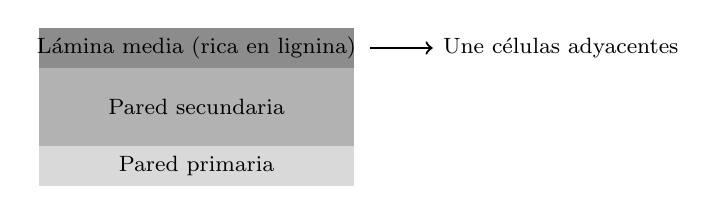
\begin{tikzpicture}
% Capas celulares
\fill[gray!30] (0,0) rectangle (4,0.5); % Pared primaria
\node[align=center] at (2,0.25) {\footnotesize Pared primaria};

\fill[gray!60] (0,0.5) rectangle (4,1.5); % Secundaria S1/S2/S3
\node[align=center] at (2,1) {\footnotesize Pared secundaria};

\fill[gray!90] (0,1.5) rectangle (4,2); % Lámina media
\node[align=center] at (2,1.75) {\footnotesize Lámina media (rica en lignina)};

% Anotación
\draw[->, thick] (4.2,1.75) -- (5,1.75) node[right] {\footnotesize Une células adyacentes};
\end{tikzpicture}

\vspace{0.5em}
\small La lignina se localiza especialmente en la lámina media y actúa como adhesivo natural.
\end{frame}

\begin{frame}{Composición Polimérica de Maderas (2025)}
\scriptsize
\centering
\renewcommand{\arraystretch}{1.2}
\begin{tabular}{|l|c|c|c|c|c|}
\hline
\textbf{Tipo de biomasa} & \textbf{Celulosa (\%)} & \textbf{Lignina (\%)} & \textbf{Glucomanano (\%)} & \textbf{Arabinogalactano (\%)} & \textbf{Xilano (\%)} \\
\hline
\textbf{Promedio frondosas}     & 42–49 & 18–25 & 2–5  & 1–3  & 20–35 \\
Álamo temblón                   & 52    & 16    & 4    & 1    & 24    \\
Haya                            & 43    & 22    & 4    & 2    & 26    \\
Abedul blanco                   & 41    & 19    & 3    & 1    & 33    \\
Arce rojo                       & 42    & 23    & 5    & 1    & 25    \\
\hline
\textbf{Promedio coníferas}     & 40–44 & 26–33 & 10–18 & 1–3  & 7–15  \\
Abeto balsámico                 & 44    & 29    & 17   & 1    & 8     \\
Cedro blanco oriental           & 43    & 30    & 11   & 2    & 11    \\
Pícea blanca                    & 44    & 28    & 17   & 3    & 7     \\
Pino de Jack                    & 42    & 30    & 16   & 2    & 10    \\
\hline
\end{tabular}
\vspace{0.5em}

\justifying
\textbf{Nota:} La celulosa representa la principal fuente estructural. Las frondosas tienen mayor xilano; las coníferas, mayor contenido de glucomanano y lignina.
\end{frame}




\begin{frame}{\textbf{Clasificación general de los combustibles}}
\begin{itemize}
  \item La clasificación es una herramienta clave para evaluar las propiedades de un combustible.
  \item Combustibles del mismo grupo tienen \textbf{comportamiento similar}, independientemente de su origen.
  \item Permite inferir el \textbf{potencial de conversión termoquímica} (ej. gasificación) de nuevas biomasas.
\end{itemize}

\textbf{Tres métodos principales de clasificación:}
\begin{enumerate}
  \item \textbf{Relaciones atómicas} (C/H/O)
  \item \textbf{Proporción de componentes lignocelulósicos} (celulosa, hemicelulosa, lignina)
  \item \textbf{Diagrama ternario} (representación gráfica de mezclas de tres componentes)
\end{enumerate}

\textit{Nota:} Solo el primer método aplica a todos los combustibles; los otros dos se aplican a biomasa lignocelulósica.
\end{frame}

\begin{frame}{\textbf{Clasificación por relación atómica}}
\begin{itemize}
  \item La relación atómica ayuda a estimar el \textbf{poder calorífico} de un combustible.
  \item El poder calorífico disminuye cuando:
  \begin{itemize}
    \item \( \uparrow \frac{O}{C} \): de 0.86 a 1.03 reduce el HHV de 20.5 a 15 MJ/kg.
    \item \(\downarrow\frac{H}{C} \): también disminuye el valor energético.
  \end{itemize}
  \item El diagrama de \textbf{van Krevelen} (H/C vs O/C) clasifica todos los combustibles en base seca libre de cenizas.
  \item Biomasa: alto contenido de H y O → \textbf{más volátiles, más gas}.
\end{itemize}

\vspace{0.5em}
\textbf{Relación lineal estimada para biomasa:}

\[
\frac{H}{C} = 1.4125 \cdot \frac{O}{C} + 0.5004
\]
\end{frame}

\begin{frame}{Diagrama de van Krevelen}
    \begin{figure}
    \centering
    
\includegraphics[width=0.65\linewidth]{Energias Alternativas/3-Biomass/img/Atomic_O_C_ratio.png}
    \caption{Clasificación de los combustibles sólidos según la relación hidrógeno/carbono y oxígeno/carbono.
Fuente: Datos de Jones et al. (2006).}
    %\label{fig:enter-label}
\end{figure}
\end{frame}

\begin{frame}{Proporciones Relativas de Componentes Lignocelulósicos}
\justifying
La biomasa también puede clasificarse según las proporciones relativas de \textbf{celulosa}, \textbf{hemicelulosa} y \textbf{lignina}. Esta clasificación es útil para predecir el comportamiento de la biomasa durante procesos térmicos como la \textbf{pirólisis}.

\vspace{1em}
Con base en estudios (Jones et al., 2006), se ha observado que:
\begin{itemize}
  \item La razón \textbf{celulosa/lignina} varía típicamente entre 0.5 y 2.7.
  \item La razón \textbf{hemicelulosa/lignina} se encuentra entre 0.5 y 2.0.
\end{itemize}

\vspace{0.5em}
Estas razones permiten identificar agrupaciones de biomasas con comportamientos térmicos similares, independientemente de su origen vegetal.
\end{frame}

\begin{frame}{Relación Celulosa/Lignina vs Hemicelulosa/Lignina}
\centering
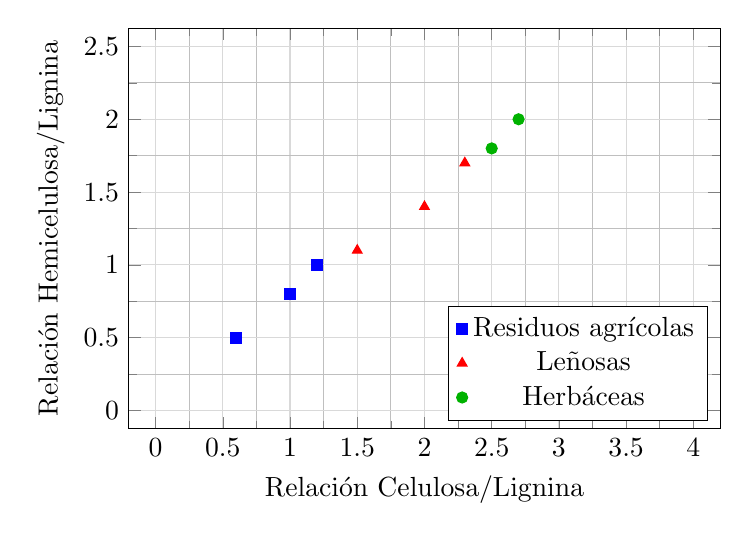
\begin{tikzpicture}
\begin{axis}[
    width=0.75\textwidth,
    height=0.55\textwidth,
    xlabel={Relación Celulosa/Lignina},
    ylabel={Relación Hemicelulosa/Lignina},
    xmin=0, xmax=4,
    ymin=0, ymax=2.5,
    grid=both,
    major grid style={gray!30},
    minor tick num=1,
    enlargelimits=0.05,
    scatter/classes={
      tipoA={mark=square*,blue},
      tipoB={mark=triangle*,red},
      tipoC={mark=*,green!70!black}
    },
    legend style={at={(0.98,0.02)}, anchor=south east},
    legend entries={Residuos agrícolas, Leñosas, Herbáceas}
]

% Datos sintéticos representativos
\addplot[scatter,only marks,scatter src=explicit symbolic]
coordinates {
  (0.6,0.5) [tipoA]
  (1.0,0.8) [tipoA]
  (1.5,1.1) [tipoB]
  (2.0,1.4) [tipoB]
  (2.5,1.8) [tipoC]
  (2.7,2.0) [tipoC]
  (1.2,1.0) [tipoA]
  (2.3,1.7) [tipoB]
};

\end{axis}
\end{tikzpicture}

\end{frame}


\begin{frame}{Diagrama Ternario C–H–O en la Gasificación de Biomasa}
\justifying
El diagrama ternario muestra la proporción atómica de Carbono (C), Hidrógeno (H) y Oxígeno (O) en combustibles sólidos como la biomasa, carbón y sus derivados. Este tipo de representación permite visualizar:
\begin{itemize}
  \item La evolución geoquímica de los combustibles sólidos hacia mayor contenido de carbono (como en el caso de la antracita).
  \item Las trayectorias de los procesos de conversión como:
    \begin{itemize}
      \item \textbf{H:} Hidrogenación
      \item \textbf{S:} Gasificación con vapor
      \item \textbf{O:} Gasificación con oxígeno
      \item \textbf{P:} Pirolisis lenta
      \item \textbf{F:} Pirolisis rápida
    \end{itemize}
  \item Biomasa moderna se ubica más cerca a los vértices de H y O que el carbón, lo que refleja su mayor contenido de hidrógeno y oxígeno.
\end{itemize}

\end{frame}


\begin{frame}{Procesos de Conversión de Biomasa en el Diagrama Ternario C–H–O}
\centering

\includegraphics[width=0.7\linewidth]{Energias Alternativas/3-Biomass/img/Diagrama_Ternario_Biomasa.png}

\scriptsize
Fuente: Adaptado de Jones et al. (2006), actualizado al 2025.
\end{frame}


\section{Propiedades de la biomasa}
\begin{frame}{\textbf{Propiedades físicas de la biomasa}}
\begin{itemize}
  \item Las propiedades físicas afectan la pirólisis y la gasificación.
  \item \textbf{Permeabilidad:} clave en pirólisis; retiene gases en los poros y favorece el craqueo secundario.
  \item Los poros de la madera están orientados \textbf{longitudinalmente}.
  \item La \textbf{conductividad térmica} y la \textbf{difusividad} varían con la dirección → comportamiento anisotrópico.
  \item La \textbf{torrefacción} puede reducir dicha anisotropía y modificar la permeabilidad.
\end{itemize}
\end{frame}
\begin{frame}{\textbf{Densidades en biomasa granular}}
\textbf{Densidades características:}
\begin{enumerate}
  \item \textbf{Densidad verdadera:} masa/volumen del contenido sólido.
  \item \textbf{Densidad aparente:} masa/volumen total incluyendo poros internos.
  \item \textbf{Densidad a granel:} masa/volumen incluyendo espacios entre partículas.
  \item \textbf{Densidad de biomasa (crecimiento):} densidad promedio natural.
\end{enumerate}

\vspace{0.5em}
\textit{Importancia:} afectan el diseño y rendimiento en procesos térmicos como combustión, gasificación o peletización.
\end{frame}
\begin{frame}{\textbf{Densidad verdadera de la biomasa}}
\begin{itemize}
  \item Se refiere al volumen ocupado únicamente por el material sólido de la biomasa.
  \item Se calcula como:
  \[
  \rho_{\text{verdadera}} = \frac{\text{masa total de la biomasa}}{\text{volumen sólido en la biomasa}}
  \]
  \item Las paredes celulares constituyen la mayor parte del contenido sólido.
  \item En madera común, la densidad de la pared celular es aproximadamente:
  \[
  1530 \text{ kg/m}^3
  \]
  \item Difícil de medir directamente → se usa \textbf{picnómetro} o se estima con el análisis último.
\end{itemize}
\end{frame}

\begin{frame}{\textbf{Densidad aparente de la biomasa}}
\begin{itemize}
  \item Basada en el \textbf{volumen externo} de la partícula, incluyendo sus poros internos.
  \item No incluye los espacios entre partículas (volumen intersticial).
  \item Se puede medir:
  \begin{itemize}
    \item Por medios mecánicos (micrómetros, calibres).
    \item Por \textbf{desplazamiento de volumen en agua}.
  \end{itemize}
  \item Se expresa como:
  \[
  \rho_{\text{aparente}} = \frac{\text{masa total de la biomasa}}{\text{volumen aparente (sólido + poros internos)}}
  \]
\end{itemize}

\vspace{0.5em}
\textbf{Uso práctico:}  
La \textbf{densidad aparente} es la más utilizada en \textbf{cálculos de diseño}, ya que:
\begin{itemize}
  \item Es fácil de medir.
  \item Representa el volumen real que ocupa una partícula dentro del sistema.
\end{itemize}

\end{frame}

\begin{frame}{\textbf{Densidad a granel de la biomasa}}
\begin{itemize}
  \item Se refiere al volumen total ocupado por un conjunto de partículas de biomasa, incluyendo:
  \begin{itemize}
    \item Sólidos
    \item Poros internos
    \item Espacios entre partículas (intersticiales)
  \end{itemize}
  \item Depende del grado de compactación del material.
  \item Se expresa como:
  \[
  \rho_{\text{granel}} = \frac{\text{masa total de las partículas de biomasa}}{\text{volumen total ocupado por las partículas}} 
  \]
\end{itemize}
\end{frame}

\begin{frame}{\textbf{Medición estandarizada de densidad a granel}}
\begin{itemize}
  \item Se utiliza el procedimiento ASTM E-873-06:
  \begin{enumerate}
    \item Verter biomasa en caja de \(305 \times 305 \times 305\ \text{mm}\) desde 610 mm.
    \item Dejar caer la caja desde 150 mm (x3) para compactar el material.
    \item Calcular:
\[
    \rho_{\text{granel}} = \frac{\text{masa final de biomasa}}{\text{volumen de la caja}}
 \]
  \end{enumerate}
  \item Se puede expresar en base:
  \begin{itemize}
    \item \textbf{Húmeda} (incluye humedad externa)
    \item \textbf{Seca en horno} (biomasa deshidratada)
  \end{itemize}
\end{itemize}
\end{frame}

\begin{frame}{\textbf{Relaciones entre densidades de la biomasa}}
\textbf{Porosidad intra-partícula:}
\[
\rho_{\text{aparente}} = \rho_{\text{verdadera}} (1 - \varepsilon_p)
\]

\textbf{Porosidad entre partículas:}
\[
\rho_{\text{granel}} = \rho_{\text{aparente}} (1 - \varepsilon_b) 
\]

\vspace{1em}
\begin{itemize}
  \item \( \varepsilon_p \): fracción de vacíos internos de una partícula.
  \item \( \varepsilon_b \): fracción de vacíos entre partículas empacadas.
  \item Permiten calcular indirectamente la densidad real del sólido.
\end{itemize}
\end{frame}

\begin{frame}{\textbf{Densidad de biomasa (crecimiento)}}
\begin{itemize}
  \item Utilizada en industrias bioenergéticas y forestales para estimar la \textbf{disponibilidad de biomasa por unidad de superficie}.
  \item Se expresa como:
  \[
  \text{toneladas secas en horno por hectárea} \quad (\text{t/ha})
  \]
  \item Incluye toda la \textbf{materia orgánica aérea viva} de:
  \begin{itemize}
    \item Hojas y ramitas
    \item Ramas y corteza
    \item Tronco principal
    \item Árboles completos
  \end{itemize}
  \item Es útil para:
  \begin{itemize}
    \item Estimar el potencial energético de un terreno
    \item Cuantificar carbono almacenado
    \item Planificar cosechas forestales o cultivos energéticos
  \end{itemize}
\end{itemize}
\end{frame}


\begin{frame}{Propiedades Termodinámicas de la Biomasa}
\justifying
\small
La gasificación es un proceso de conversión termoquímica, por lo tanto, las propiedades termodinámicas de la biomasa influyen significativamente en su comportamiento durante este proceso.

Entre las propiedades más importantes para el diseño y análisis de sistemas de gasificación se encuentran:

\begin{itemize}
    \item \textbf{Conductividad térmica:} mide la capacidad de la biomasa para conducir calor, afectando la velocidad de transferencia térmica durante el calentamiento.
    
    \item \textbf{Calor específico:} representa la cantidad de energía necesaria para aumentar la temperatura de una unidad de masa de biomasa en un grado Celsius.
    
    \item \textbf{Entalpía de formación:} corresponde a la cantidad de energía absorbida o liberada cuando la biomasa se forma a partir de sus elementos constituyentes.
\end{itemize}

Estas propiedades dependen de la composición química, la densidad aparente, el contenido de humedad y la estructura interna de la biomasa.


\end{frame}




\begin{frame}{\textbf{Conductividad t\'ermica de la biomasa}}
\begin{itemize}
  \item La biomasa es anisotr\'opica: su conductividad t\'ermica depende de:
  \begin{itemize}
    \item Direcci\'on (a lo largo o transversal a la fibra)
    \item Humedad y densidad
    \item Temperatura y porosidad
  \end{itemize}
  \item Influye directamente en la pir\'olisis y gasificaci\'on
\end{itemize}

\textbf{Correlaci\'on emp\'irica de MacLean (1941):}

\[
K_{\text{eff}}(W/m K) =
\begin{cases}
\text{sp.gr} \cdot (0.21 - 0.004 \cdot md) + 0.0238, & md > 40\% \\
\text{sp.gr} \cdot (0.21 - 0.0055 \cdot md) + 0.0238, & md \leq 40\%
\end{cases}
\]

\begin{itemize}
  \item \textbf{sp.gr}: gravedad espec\'ifica de la biomasa (relaci\'on entre densidad del s\'olido y la del agua).
  \item \textbf{md}: porcentaje de humedad en base seca (\% en base seca, dry basis (db)).
\end{itemize}
\end{frame}

\begin{frame}{\textbf{Modelo direccional y componentes}} 
\textbf{Conductividad t\'ermica efectiva paralela a la fibra:}
\[
K_{\text{eff}}(W/m K) = G(x) K_s + F(x) K_w + H(x) (K_g + K_{\text{rad}})
\]

\textbf{Donde:}
\begin{itemize}
  \item \( G(x) \): fracci\'on de volumen de la pared celular seca.
  \item \( F(x) \): fracci\'on de volumen de la humedad en la celda.
  \item \( H(x) \): fracci\'on de volumen de gas en los poros.
\end{itemize}

\textbf{Contribuciones individuales:}
\[
\begin{aligned}
K_w &=-0.487 + 5.887\times10^{-3}T - 7.393\times10^{-6}T^2 \\
K_g &= -7.494\times10^{-3} + 1.709\times10^{-4}T - 2.377\times10^{-7}T^2 \\ &\quad + 2.202\times10^{-10}T^3 - 9.463\times10^{-14}T^4 + 1.581\times10^{-17}T^5 \\
K_s &= 0.52 \quad \text{(transversal a la fibra)}
\end{aligned}
\]
\end{frame}

\begin{frame}{Conductividad Térmica Direccional en Biomasa}
\small
\justifying
Para simular procesos termoquímicos como la \textbf{pirolisis}, \textbf{gasificación} o \textbf{combustión}, es esencial conocer la conductividad térmica en distintas direcciones de la biomasa.

\textbf{1. Conductividad en pared celular (dirección paralela):}
\[
K_w = 20.487 - 5.887 \times 10^{-3} T + 7.393 \times 10^{-6} T^2
\]

\textbf{2. Conductividad del gas en poros:}
\[
K_g = 27.494 \times 10^{-3} - 11.709 \times 10^{-4} T + \cdots - 1.581 \times 10^{-17} T^5
\]

\textbf{3. Conductividad perpendicular a la fibra:}
\[
K_s = 0.52 \quad (\text{constante})
\]

\end{frame}





\begin{frame}{\textbf{Conducci\'on radiativa y resumen}}
\textbf{4. Radiación en poros (importante a alta T):}
\[
K_{\text{rad}} = 5.33 \cdot \varepsilon_{\text{rad}} \cdot \sigma \cdot T^3 \cdot d_{\text{pore}}
\]

\textbf{Donde:} \(\varepsilon_{\text{rad}}\) es la emisividad, \(\sigma = 5.67 \times 10^{-8} \, \text{W/m}^2\text{K}^4\), \(T\) en K, y \(d_{\text{pore}}\) el diámetro del poro (m).


\begin{itemize}
  \item Importante a altas temperaturas
  \item Aporta en gasificaci\'on a alta T
\end{itemize}

\vspace{0.5em}
\textbf{Tendencias:}
\begin{itemize}
  \item Conductividad \(\uparrow\) con densidad seca
  \item Mayor en maderas duras (mayor densidad)
  \item \textbf{A lo largo de la fibra} > transversal
\end{itemize}
\end{frame}

\begin{frame}{\textbf{Calor espec\'ifico}}
\begin{itemize}
  \item Es una propiedad termodin\'amica esencial en los c\'alculos energ\'eticos.
  \item Representa la capacidad de almacenamiento de calor de la biomasa.
  \item Afectado por la \textbf{temperatura} y \textbf{humedad}, pero no significativamente por la densidad o especie de madera.
  \item La corteza suele tener calor espec\'ifico mayor que la madera interna.
  \item El carb\'on (char) derivado de biomasa tiene calor espec\'ifico significativamente m\'as bajo.
\end{itemize}
\end{frame}

\begin{frame}{\textbf{Entalp\'ia de formaci\'on}}
\begin{itemize}
  \item Es el cambio de entalp\'ia cuando se forma 1 mol de un compuesto desde sus elementos en estado est\'andar (25\,\textdegree C, 1 atm).
  \item Por convenci\'on, los elementos en su estado est\'andar tienen entalp\'ia de formaci\'on cero.
  \item Ejemplo:
\end{itemize}

\[
\text{H}_2 (gas) + 0.5\text{O}_2 (gas) = \text{H}_2\text{O} (gas)  -241.5 \text{ kJ/mol} 
\]

\begin{itemize}
  \item El signo negativo indica una reacci\'on exot\'ermica.
  \item Si la formaci\'on ocurre en varios pasos, la entalp\'ia total es la suma de los cambios en cada paso.
  \item Gases como H$_2$, O$_2$, N$_2$ y Cl$_2$ tienen entalp\'ia de formaci\'on igual a cero.
\end{itemize}
\end{frame}

\begin{frame}{\textbf{Calor de combusti\'on (reacci\'on)}}
\begin{itemize}
  \item El \textbf{calor de reacci\'on} (HR) es el calor liberado o absorbido en una reacci\'on qu\'imica, sin cambio de temperatura.
  \item En reacciones de combusti\'on, se denomina \textbf{calor de combusti\'on} \( \Delta H_{\text{comb}} \).
  \item Se puede calcular a partir del \textbf{calor de formaci\'on} \( H_f \).
\end{itemize}

\textbf{Ejemplo de reacci\'on de combusti\'on:}
\[
\text{CH}_4 + {2} \text{O}_2 \rightarrow 2 \text{H}_2\text{O} + \text{CO}_2
\]

\textbf{C\'alculo de} \( \Delta H_{\text{comb}} \):
\[
\Delta H_{\text{comb}} = 2 \Delta H_{\text{H}_2\text{O}} + \Delta H_{\text{CO}_2} - \Delta H_{\text{CH}_4} - {2} \Delta H_{\text{O}_2} 
\]

\begin{itemize}
  \item Tambi\'en puede definirse como el \textbf{cambio de entalp\'ia} de la reacci\'on de combusti\'on cuando est\'a balanceada:
\[
\text{Combustible} + \text{O}_2 \rightarrow \text{H}_2\text{O} + \text{CO}_2 - HR
\]
\end{itemize}
\end{frame}
\begin{frame}{\textbf{Ejemplo}}
Encuentre el \textbf{calor de formación del aserrín}, cuyo poder calorífico se da como \( 476\, \text{kJ/mol}
\)
Suponga que su fórmula química es:
\(
\text{CH}_{1.35}\text{O}_{0.617}
\)
\begin{table}[h!]
\centering
\caption{\textbf{Calor de formaci\'on de algunos compuestos importantes a 25\textdegree C}}
\scriptsize
\begin{tabular}{|c|c|c|c|c|c|c|c|}
\hline
\textbf{Compuesto} & H$_2$O & CO$_2$ & CO & CH$_4$ & O$_2$ & CaCO$_3$ & NH$_3$ \\
\hline
\textbf{Calor de formaci\'on (kJ/mol)} & -241.5 & -393.5 & -110.6 & -74.8 & 0 & -1211.8 & -82.5 \\
\hline
\end{tabular}
\\[0.5em]
\footnotesize Fuente: Datos tomados de Perry y Green (1997, p\'ags. 2--186).
\end{table}
\textbf{Calor de combusti\'on (reacci\'on)}
\begin{itemize}
  \item El \textbf{calor de reacci\'on} (HR) es el calor liberado o absorbido en una reacci\'on qu\'imica, sin cambio de temperatura.
  \item En reacciones de combusti\'on, se denomina \textbf{calor de combusti\'on} \( \Delta H_{\text{comb}} \).
  \item Se puede calcular a partir del \textbf{calor de formaci\'on} \( H_f \).
\end{itemize}

\end{frame}
\begin{frame}{\textbf{Datos iniciales}}
\begin{itemize}
  \item \textbf{F\'ormula emp\'irica del aserr\'in:} \( \text{CH}_{1.35}\text{O}_{0.617} \)
  \item \textbf{Calor de combusti\'on:} \( \Delta H_{\text{comb}} = 476\, \text{kJ/mol} \)
\end{itemize}

{\textbf{Paso 1: Ecuaci\'on de combusti\'on balanceada}}
\[
\text{CH}_{1.35}\text{O}_{0.617} + 1.029\, \text{O}_2 \rightarrow \text{CO}_2 + 0.675\, \text{H}_2\text{O} -476 kJ/mol
\]


\begin{itemize}
  \item El carbono genera 1 mol de CO$_2$
  \item Los 1.35 \'atomos de H producen \( \frac{1.35}{2} = 0.675 \) mol de H$_2$O 
\end{itemize}


\[
HR =[HF_{Co_2}+0.675HF_{H_2O}]-[HF_{sw}+1.029HF_{O_2}]
\]
\end{frame}
\begin{frame}{\textbf{Calor de reacci\'on mediante entalp\'ias}}
\begin{itemize}
  \item \( H_F(\text{CO}_2) = -393.5\, \text{kJ/mol} \)
  \item \(  H_F(\text{H}_2\text{O}) = -241.5\, \text{kJ/mol} \)
  \item \( H_F(\text{O}_2) = 0\, \text{kJ/mol} \)
\end{itemize}

\[
HR_{sw} = \left[ -393.5 + 0.675 \cdot (-241.5) \right] - HF_{sw}
\]
\[
HR_{sw}=-556.5 - HF_{sw}
\]
\[
HF_{sw}-556.5-(-476)= -80.5 kJ/mol
\]


\end{frame}
\begin{frame}{\textbf{Poder calor\'ifico} (Heating Value) }
\begin{itemize}
  \item El poder calor\'ifico de la biomasa es la cantidad de energ\'ia que libera cuando se quema completamente con ox\'igeno suficiente.
  \item Es una de las propiedades m\'as importantes en procesos de conversi\'on energ\'etica.
  \item En comparaci\'on con combustibles f\'osiles, la biomasa tiene un poder calor\'ifico m\'as bajo, especialmente en base volum\'etrica.
  \item Esto se debe a:
  \begin{itemize}
    \item Su baja densidad
    \item Su alto contenido de ox\'igeno
  \end{itemize}
\end{itemize}
\end{frame}
\begin{frame}{\textbf{Composici\'on de la biomasa}}
La biomasa contiene una gran cantidad de compuestos org\'anicos complejos, humedad (\textbf{M}) y una peque\~na cantidad de impurezas inorg\'anicas conocidas como \textbf{cenizas} (\textbf{ASH}).

Los compuestos org\'anicos est\'an formados por cuatro elementos principales:
\begin{itemize}
    \item Carbono (C)
    \item Hid\'rogeno (H)
    \item Ox\'igeno (O)
    \item Nitr\'ogeno (N)
\end{itemize}

La biomasa (por ejemplo, residuos s\'olidos municipales y desechos animales) tambi\'en puede contener peque\~nas cantidades de cloro (Cl) y azufre (S). El azufre rara vez est\'a presente, excepto en fuentes secundarias como madera de demolici\'on.

\end{frame}

\begin{frame}{\textbf{Composici\'on para dise\~no t\'ermico}}
El dise\~no t\'ermico de un sistema de aprovechamiento de biomasa (gasificador o combustor) requiere conocer:
\begin{itemize}
    \item La composici\'on del combustible
    \item Su contenido energ\'etico
\end{itemize}

En el contexto de la conversi\'on t\'ermica como la combusti\'on, se utilizan principalmente:
\begin{enumerate}
    \item Composici\'on \textbf{\'ultima} o \textbf{elemental}
    \item Composici\'on \textbf{pr\'oxima}
\end{enumerate}

Adem\'as, existe la \textbf{composici\'on polim\'erica} importante en procesos como la torrefacci\'on, pir\'olisis y gasificaci\'on.
\end{frame}




\begin{frame}{\textbf{An\'alisis \'Ultimo}}
El an\'alisis \textbf{\'ultimo} expresa la composici\'on de un combustible en t\'erminos de sus \'elementos b\'asicos, excluyendo humedad (\textbf{M}) y cenizas inorg\'anicas (\textbf{ASH}).

\[
C+H+O+N+S+ASH+M = 100\% 
\]

\begin{itemize}
  \item \textbf{C, H, O, N, S}: Porcentajes en masa de carbono, hidr\'ogeno, ox\'igeno, nitr\'ogeno y azufre
  \item La humedad (M) se informa por separado
  \item El H y O aqu\'i corresponden solo a la materia org\'anica, no al agua
\end{itemize}

La mayor\'ia de las biomasas no contiene azufre (S).
\end{frame}

\begin{frame}{\textbf{Ratios at\'omicos y contenido energ\'etico}}
\begin{itemize}
  \item Los cocientes \( \text{H/C} \) y \( \text{O/C} \) se derivan del an\'alisis \'ultimo
  \item La biomasa, especialmente la celulosa, tiene altos contenidos de H y O
  \item Esto implica un \textbf{bajo poder calor\'ifico} comparado con combustibles f\'osiles
\end{itemize}


\textbf{Contenido de azufre y emisiones}
\begin{itemize}
  \item La biomasa lignocelul\'osica tiene \textbf{muy bajo contenido de azufre}
  \item Esto reduce las emisiones de SO$_2$ al utilizarse como combustible
  \item Para combustibles con S (carb\'on, fuel-oil), se usa CaCO$_3$ para capturarlo
  \item Cada mol de azufre capturado libera 1 mol de CO$_2$ adicional
\end{itemize}
\end{frame}

\begin{frame}{\textbf{Beneficio ambiental de la biomasa}}
\begin{itemize}
  \item La biomasa es \textbf{neutra en carbono (CO$_2$)}
  \item Evita emisiones adicionales de CO$_2$ asociadas a la captura de SO$_2$
  \item Por tanto, su uso en lugar de combustibles f\'osiles reduce a\'un m\'as las emisiones de gases contaminantes
\end{itemize}
\end{frame}

\begin{frame}{Análisis Último (base seca) de Biomasas}
\scriptsize
\centering
\begin{tabular}{lccccccc}
\toprule
\textbf{Biomasa} & \textbf{C (\%)} & \textbf{H (\%)} & \textbf{N (\%)} & \textbf{S (\%)} & \textbf{O (\%)} & \textbf{Cenizas (\%)} & \textbf{HHV (kJ/kg)} \\
\midrule
Arce (Maple)            & 50.6 & 6.0 & 0.3 & 0.0 & 41.7 & 1.4 & 19,958 \\
Abeto Douglas           & 52.3 & 6.3 & 9.1 & 0.0 & 40.5 & 0.8 & 21,051 \\
Abeto Douglas (corteza) & 56.2 & 5.9 & 0.0 & 0.0 & 36.7 & 1.2 & 22,098 \\
Secuoya (Redwood)       & 53.5 & 5.9 & 0.1 & 0.0 & 40.3 & 0.2 & 21,028 \\
Desecho de secuoya      & 53.4 & 6.0 & 39.9 & 0.1 & 0.1 & 0.6 & 21,314 \\
Lodos de depuradora     & 29.2 & 3.8 & 4.1 & 0.7 & 19.9 & 42.1 & 16,000 \\
Paja de arroz           & 39.2 & 5.1 & 0.6 & 0.1 & 35.8 & 19.2 & 15,213 \\
Cáscara de arroz        & 38.5 & 5.7 & 0.5 & 0.0 & 39.8 & 15.5 & 15,376 \\
Madera residual (SW)    & 47.2 & 6.5 & 0.0 & 0.0 & 45.4 & 1.0 & 20,502 \\
Papel                   & 43.4 & 5.8 & 0.3 & 0.2 & 44.3 & 6.0 & 17,613 \\
RSU (MSW)               & 47.6 & 6.0 & 1.2 & 0.3 & 32.9 & 12.0 & 19,879 \\
Desechos animales       & 42.7 & 5.5 & 2.4 & 0.3 & 31.3 & 17.8 & 17,167 \\
\bottomrule
\end{tabular}

\vspace{0.8em}
\scriptsize{Fuente: Adaptado de Reed (2002) y Tillman (1978).}
\end{frame}


\begin{frame}{Análisis Último (base seca) de Combustibles Fósiles}
\scriptsize
\centering
\begin{tabular}{lccccccc}
\toprule
\textbf{Combustible} & \textbf{C (\%)} & \textbf{H (\%)} & \textbf{N (\%)} & \textbf{S (\%)} & \textbf{O (\%)} & \textbf{Cenizas (\%)} & \textbf{HHV (kJ/kg)} \\
\midrule
Turba (Peat)          & 54.5 & 5.1 & 1.65 & 0.45 & 33.09 & 5.2  & 21,230 \\
Lignito               & 62.5 & 4.38 & 0.94 & 1.41 & 17.2  & 13.4 & 24,451 \\
Carbón PRB            & 65.8 & 4.88 & 0.86 & 1.0  & 16.2  & 11.2 & 26,436 \\
Antracita             & 83.7 & 1.9  & 0.9  & 0.7  & 10.5  & 2.3  & 27,656 \\
Petcoke               & 82.0 & 0.5  & 0.7  & 0.8  & 10.0  & 6.0  & 28,377 \\
\bottomrule
\end{tabular}

\vspace{0.8em}
\scriptsize{Fuente: Adaptado de Reed (2002), Basu et al. (2000) y Probstein y Hicks (2006).}
\end{frame}












\begin{frame}{\textbf{An\'alisis Pr\'oximo}}
El an\'alisis pr\'oximo proporciona la composici\'on de la biomasa en t\'erminos de:
\begin{itemize}
    \item Humedad (M)
    \item Materia vol\'atil (VM)
    \item Cenizas (ASH)
    \item Carbono fijo (FC)
\end{itemize}
Es un procedimiento relativamente sencillo y econ\'omico.


\textbf{Materia vol\'atil}
\begin{itemize}
    \item Vapores condensables y no condensables liberados al calentar el combustible.
    \item Su cantidad depende de:
    \begin{itemize}
        \item Velocidad de calentamiento
        \item Temperatura alcanzada
    \end{itemize}
\end{itemize}
\end{frame}

\begin{frame}{\textbf{Cenizas} (Ash)}
\begin{itemize}
    \item Residuos inorg\'anicos s\'olidos tras la combusti\'on total del combustible.
    \item Componentes principales: s\'ilice, aluminio, hierro y calcio.
    \item Otros presentes en menor cantidad: magnesio, titanio, sodio y potasio.
    \item Algunas cenizas pueden oxidarse al quemar; puede requerir correcci\'on.
\end{itemize}

\textbf{Importancia de las cenizas (Ash)}
\begin{itemize}
    \item La biomasa suele tener bajo contenido de cenizas.
    \item Puede ser significativo si contiene:
    \begin{itemize}
        \item Metales alcalinos (p. ej. potasio)
        \item Hal\'ogenos (p. ej. cloro)
    \end{itemize}
    \item Problem\'aticos en paja, pastos y madera de demolici\'on.
    \item Riesgo de: aglomeraci\'on, incrustaciones, corrosi\'on en calderas o gasificadores.
\end{itemize}
\end{frame}

\begin{frame}{\textbf{Origen adicional de las cenizas}}
\begin{itemize}
    \item No siempre provienen de la biomasa en s\'i.
    \item Durante su recolecci\'on y manipulaci\'on puede contaminarse con:
    \begin{itemize}
        \item Tierra
        \item Piedras
        \item Impurezas
    \end{itemize}
    \item En muchas plantas, estas impurezas son el principal componente inorg\'anico del insumo de biomasa.
\end{itemize}
\end{frame}
\begin{frame}{\textbf{Humedad en la biomasa}}
\begin{itemize}
    \item La biomasa presenta caracter\'isticamente un alto contenido de humedad.
    \item Las ra\'ices absorben agua y la transportan al duramen y luego a las hojas.
    \item Parte se usa en la fotos\'intesis y el resto se libera por transpiraci\'on.
    \item \textbf{Las hojas contienen m\'as humedad que el tronco.}
\end{itemize}


\textbf{Contenido total de humedad}
\begin{itemize}
    \item Puede alcanzar hasta el \textbf{90\% (base seca)}.
    \item Drena energ\'ia aprovechable, ya que \textbf{la evaporaci\'on no recupera energ\'ia}.
    \item Es un par\'ametro clave para:
    \begin{itemize}
        \item Evaluar costos de transporte
        \item Penalizaci\'on energ\'etica del secado
    \end{itemize}
\end{itemize}
\end{frame}

\begin{frame}{\textbf{Formas de humedad en biomasa}}
\begin{itemize}
    \item \textbf{Humedad libre o externa:} por fuera de las paredes celulares.
    \item \textbf{Humedad inherente o de equilibrio:} absorbida dentro de las paredes celulares.
    \item Cuando las paredes est\'an saturadas: se alcanza el \textbf{punto de saturaci\'on de fibra}.
\end{itemize}
\textbf{Humedad de equilibrio y condiciones ambientales}
\begin{itemize}
    \item Depende fuertemente de la \textbf{humedad relativa} del aire.
    \item Tiene baja dependencia con la temperatura del aire.
    \item Ejemplo: en la madera, la humedad de equilibrio var\'ia del 3\% al 27\% cuando la HR sube del 10\% al 80\%.
    \item Fuente: Kitani y Hall (1989, p. 864)
\end{itemize}
\end{frame}
\begin{frame}{\textbf{Expresi\'on de la humedad en biomasa}}
\begin{itemize}
    \item La humedad de la biomasa se suele expresar en \textbf{base seca}.
    \item Si \( W_{\text{wet}} \) es la masa h\'umeda y \( W_{\text{dry}} \) la masa seca:
\end{itemize}
\[
M_{\text{dry}} = \frac{W_{\text{wet}} - W_{\text{dry}}}{W_{\text{dry}}} 
\]
\begin{itemize}
    \item Esta expresi\'on puede superar el 100\% para biomasa muy h\'umeda.
    \item Por ello, \textbf{siempre debe especificarse la base usada}.
\end{itemize}
\end{frame}

\begin{frame}{\textbf{Humedad en base h\'umeda y relaci\'on con base seca}}
\begin{itemize}
    \item Humedad en \textbf{base h\'umeda}:
\end{itemize}
\[
M_{\text{wet}} = \frac{W_{\text{wet}} - W_{\text{dry}}}{W_{\text{wet}}} 
\]
\begin{itemize}
    \item Relaci\'on entre ambas:
\end{itemize}
\[
M_{\text{dry}} = \frac{M_{\text{wet}}}{1 - M_{\text{wet}}}
\]
\end{frame}

\begin{frame}{\textbf{Carbono Fijo en Biomasa}}
\small
\begin{itemize}
    \item El \textbf{carbono fijo (FC)} representa el carbono s\'olido que permanece tras la devolatilizaci\'on.
    \item Se calcula mediante:
\end{itemize}
\(
FC = 1 - M - VM - ASH 
\)
\begin{itemize}
    \item Donde M es humedad, VM es materia vol\'atil, y ASH son cenizas.
\end{itemize}
\textbf{Origen y determinaci\'on del FC}
\begin{itemize}
    \item En carb\'on: incluye carbono elemental + residuos carbonosos de la medici\'on de VM.
    \item En biomasa: todo el carbono es \textbf{org\'anico}, fijado por fotos\'intesis.
    \item Parte del carbono org\'anico se convierte en \textbf{carbono pirol\'itico} durante la medici\'on de VM.
    \item El FC \textbf{no se mide directamente}, depende de la VM.
\end{itemize}
\end{frame}

\begin{frame}{\textbf{Importancia del FC en gasificaci\'on}}
\begin{itemize}
    \item La velocidad y el rendimiento de gasificaci\'on dependen de la conversi\'on del FC.
    \item Esta reacci\'on es la m\'as lenta y determina el \textbf{tama\~no del gasificador}.
    \item Aunque se llama "carbono fijo", \textbf{no es una cantidad fija}; depende de las condiciones de medici\'on.
\end{itemize}
\textbf{Char: carb\'on pirol\'itico}
\begin{itemize}
    \item El char es un residuo carbonoso de la \textbf{pir\'olisis}, pero no es carbono puro ni el FC exacto.
    \item Contiene:
    \begin{itemize}
        \item Vol\'atiles
        \item Cenizas
        \item Carbono fijo
    \end{itemize}
    \item Es muy reactivo, altamente poroso y \textbf{no se apelmaza}.
\end{itemize}
\end{frame}

\begin{frame}{\textbf{An\'alisis Termogravim\'etrico}}
\begin{itemize}
    \item El an\'alisis pr\'oximo seg\'un la norma ASTM D-3172 puede ser costoso y lento.
    \item Klass (1998) propuso una alternativa usando:
    \begin{itemize}
        \item \textbf{Termogravimetr\'ia (TG)}
        \item \textbf{Termogravimetr\'ia diferencial (DTG)}
    \end{itemize}
\end{itemize}

\textbf{Bases para expresar la composici\'on de la biomasa}
\begin{itemize}
    \item La composici\'on del combustible puede expresarse en diferentes bases seg\'un la aplicaci\'on.
    \item Las cuatro bases m\'as comunes son:
    \begin{enumerate}
        \item Tal como se recibe (\textit{as-received})
        \item Seco al aire (\textit{air-dry})
        \item Totalmente seco (\textit{total dry})
        \item Seco y libre de cenizas (\textit{dry and ash-free})
    \end{enumerate}
\end{itemize}
\end{frame}
\begin{frame}{Composición básica de biomasa}
    \begin{figure}
    \centering
    
\includegraphics[width=1\linewidth]{Energias Alternativas/3-Biomass/img/comp_basic_biommasa.png}
  %  \caption{}
    %\label{fig:enter-label}
\end{figure}
\end{frame}

\begin{frame}{\textbf{Base tal como se recibe (As-Received)}}
\begin{itemize}
    \item En esta base, los resultados de los an\'alisis \textbf{pr\'oximo} y \textbf{\'ultimo} incluyen la humedad y las cenizas.
\end{itemize}

\textbf{An\'alisis \'ultimo:}
\(
C + H + O + N + S + ASH + M = 100\% 
\)

\textbf{An\'alisis pr\'oximo:}
\(
VM + FC + M + ASH = 100\% 
\)

\begin{itemize}
    \item VM: Materia vol\'atil
    \item FC: Carbono fijo
    \item M: Humedad
    \item ASH: Cenizas
\end{itemize}

\begin{itemize}
    \item \textbf{Nota:} El contenido de humedad y cenizas es el mismo en ambos an\'alisis.
    \item Esta base puede convertirse en otras como seco al aire, totalmente seco o seco y libre de cenizas.
\end{itemize}
\end{frame}

\begin{frame}{\textbf{Base seco al aire (Air-Dry)}}
\begin{itemize}
    \item En esta base se elimina solo la \textbf{humedad superficial}, conservando la humedad inherente.
    \item Para expresar un componente en base seco al aire (\textbf{ad}), se divide su valor entre la masa total menos la humedad superficial.
\end{itemize}

\textbf{Ejemplo: porcentaje de carbono en base seco al aire:}
\[
C_{ad} = \frac{100 \cdot C}{100 - M_a} 
\]

\begin{itemize}
    \item $C$: porcentaje de carbono en la muestra h\'umeda.
    \item $M_a$: masa de la humedad superficial eliminada tras el secado al aire (por cada 100 kg de combustible h\'umedo).
    \item Los dem\'as componentes del combustible se calculan de forma similar.
\end{itemize}
\end{frame}

\begin{frame}{\textbf{Base totalmente seca (Total Dry)}}
\begin{itemize}
    \item La base \textbf{seco al aire (ad)} es f\'acil de medir, pero no elimina la humedad inherente.
    \item Para expresar la composici\'on del combustible en base \textbf{totalmente seca (td)}, se considera toda la humedad: superficial e inherente.
\end{itemize}

\textbf{Porcentaje de carbono en base totalmente seca:}
\[
C_{td} = \frac{100 \cdot C}{100 - M_i} 
\]

\begin{itemize}
    \item $C$: porcentaje de carbono en el combustible h\'umedo.
    \item $M_i$: humedad inherente.
    \item La humedad total del combustible se calcula como: \( M = M_a + M_i \)
\end{itemize}
\end{frame}

\begin{frame}{\textbf{3.6.4.4 Base seca y libre de cenizas (Dry Ash-Free)}}
\begin{itemize}
    \item En esta base se eliminan tanto la \textbf{humedad} como las \textbf{cenizas (ASH)}.
    \item La composici\'on del combustible se expresa considerando solo la masa \textbf{org\'anica}.
\end{itemize}

\textbf{Porcentaje de carbono en base seca y libre de cenizas:}
\[
C_{daf} = \frac{100 \cdot C}{100 - M - ASH} 
\]

\begin{itemize}
    \item $M$: humedad total
    \item $ASH$: porcentaje de cenizas
    \item $100 - M - ASH$: masa seca y libre de cenizas
\end{itemize}

\textbf{Relaci\'on en cualquier base el total es 100 por ejemplo:}
\[
C_{daf} + H_{daf} + O_{daf} + N_{daf} + S_{daf} = 100\% 
\]
\end{frame}

\begin{frame}{\textbf{3.6.5 Poder calor\'ifico del combustible}}
\begin{itemize}
    \item El poder calor\'ifico de la biomasa es relativamente bajo, especialmente en base volum\'etrica,
    \item Esto se debe a que su \textbf{densidad es muy baja}.
\end{itemize}
\end{frame}

\begin{frame}{\textbf{Poder Calor\'ifico Superior (HHV)}}
\begin{itemize}
    \item Se define como la cantidad de calor liberado por unidad de masa o volumen de combustible.
    \item Cuando se quema completamente a 25\,\textdegree C y los productos retornan a esa temperatura.
    \item Incluye el \textbf{calor latente de vaporizaci\'on del agua}.
    \item Tambi\'en se conoce como \textbf{poder calor\'ifico bruto}.
    \item En Norteam\'erica, la eficiencia t\'ermica de los sistemas se expresa com\'unmente en t\'erminos de HHV.
    \item Por ello, es importante conocer el HHV del combustible de dise\~no.
\end{itemize}
\end{frame}

\begin{frame}
\frametitle{Poder Calorífico Inferior (LHV)}

\begin{itemize}
  \item La temperatura de los gases de escape de una caldera suele estar entre 120 y 180 °C.
  \item El vapor de agua generado en la combustión no se condensa, por lo tanto, no se recupera su calor latente de vaporización.
  \item El calor útil disponible es menor que el HHV.
  \item El LHV se define como:
\end{itemize}

\[
LHV = HHV - h_g \cdot \left( \frac{9H}{100} + \frac{M}{100} \right)
\]

\begin{itemize}
  \item Donde:
  \begin{itemize}
    \item $HHV$: Poder calorífico superior
    \item $H$: Porcentaje de hidrógeno (base "as-received")
    \item $M$: Porcentaje de humedad
    \item $h_g$: Calor latente del vapor ($2260 \, \text{kJ/kg}$)
  \end{itemize}
\end{itemize}

\end{frame}

\begin{frame}
\frametitle{Bases para expresar el Poder Calorífico}

\begin{itemize}
    \item El poder calorífico (HHV o LHV) puede expresarse en distintas bases:
    \begin{itemize}
        \item \textbf{ar}: tal como se recibe (*as-received*)
        \item \textbf{db}: base seca, también conocida como libre de humedad (*dry basis*)
        \item \textbf{daf}: base seca y libre de cenizas (*dry ash-free*)
    \end{itemize}
\end{itemize}

\vspace{0.5cm}

Si una masa \( M_f \) de combustible contiene:
\begin{itemize}
    \item \( Q \) kJ de energía total
    \item \( M_w \) kg de humedad
    \item \( M_{ash} \) kg de cenizas
\end{itemize}

\end{frame}

\begin{frame}
\frametitle{Cálculo del HHV en diferentes bases}

\[
\text{HHV}_{ar} = \frac{Q}{M_f} \quad \text{kJ/kg}
\]
\[
\text{HHV}_{db} = \frac{Q}{M_f - M_w} \quad \text{kJ/kg}
\]
\[
\text{HHV}_{daf} = \frac{Q}{M_f - M_w - M_{ash}} \quad \text{kJ/kg}
\]

\bigskip

\begin{itemize}
    \item Estas conversiones son esenciales para comparar biomasas con diferentes contenidos de humedad y ceniza.
\end{itemize}

\end{frame}


\begin{frame}
\frametitle{Métodos de estimación del HHV}

\begin{itemize}
    \item El poder calorífico puede obtenerse experimentalmente (método más confiable).
    \item Si no se puede medir, se emplean correlaciones empíricas.
    \item Una de las más conocidas es la de Channiwala y Parikh (2002):
\end{itemize}

\[
\text{HHV} = 349.1C + 1178.3H + 100.5S - 103.4O - 15.1N - 21.1 \, \text{ASH} \quad \text{(kJ/kg)}
\]

\begin{itemize}
    \item Donde C, H, S, O, N y ASH son porcentajes en peso sobre base seca.
\end{itemize}

\end{frame}

\begin{frame}
\frametitle{Rangos válidos y método alternativo}

\textbf{Rangos de validez de la correlación:}

\begin{itemize}
    \item \(0 < C < 92\%\), \(0.43 < H < 25\%\)
    \item \(0 < O < 50\%\), \(0 < N < 5.6\%\)
    \item \(0 < ASH < 71\%\), \(4745 < HHV < 55345 \, \text{kJ/kg}\)
\end{itemize}

\vspace{0.3cm}
\textbf{Método alternativo de Zhu y Venderbosch (2005):}

\[
\text{HHV} = 3220 \cdot SR \quad \text{(kJ/kg)}
\]

\begin{itemize}
    \item \(SR\): masa teórica de aire necesaria para quemar 1 kg de combustible
    \item Útil para diseño preliminar sin análisis último
\end{itemize}

\end{frame}

\begin{frame}
\frametitle{Aire seco requerido para combustión completa}

\begin{itemize}
    \item El aire seco contiene aproximadamente:
    \begin{itemize}
        \item 23.16\% de oxígeno
        \item 76.8\% de nitrógeno
        \item 0.04\% de gases inertes
    \end{itemize}
    
    \item El aire seco requerido para combustión completa de 1 kg de hidrocarburo seco:
\end{itemize}
\[
M_{da} = 0.1153 \cdot C + 0.3434 ( H - \frac{O}{8} + 0.043  S)
\quad \text{(kg de aire seco / kg de combustible seco)}
\]

\begin{itemize}
    \item Donde: $C$, $H$, $O$, $S$ son los porcentajes en peso sobre base seca.
    \item \(M_{da}\): Masa de aire seco necesaria para la combustión completa.
\end{itemize}

\end{frame}


\begin{frame}{\textbf{Aire real con exceso y humedad}}
\justifying
Para procesos reales, el aire suministrado se incrementa con un factor de exceso de aire (\(EAC\)) y humedad (\(X_m\)):

\vspace{1em}
\[
M_{wa} = (1 + EAC) \cdot M_{da} \cdot (1 + X_m)
\quad \text{[kg aire húmedo / kg combustible seco]}
\]

\vspace{1em}
\textbf{Donde:}
\begin{itemize}
  \item \(EAC\): Fracción de exceso de aire (por ejemplo, 0.2 para 20 %)
  \item \(X_m\): Fracción de humedad en el aire (por ejemplo, 0.015)
  \item \(M_{wa}\): Masa total de aire real (húmedo) requerido
\end{itemize}

\vspace{0.5em}
Este cálculo es esencial para el diseño de sistemas de combustión y optimización de calderas y hornos industriales en 2025.
\end{frame}



\begin{frame}
\frametitle{Cálculo de gases producto de la combustión completa}

\begin{itemize}
    \item El peso total de los gases de combustión generados por la combustión de 1 kg de biomasa se calcula mediante:
\end{itemize}

\[
W_c = M_{wa} - 0.2315 \cdot M_{da} + 3.66C + 9H + N + O + 2.5S \tag{3.33}
\]

\begin{itemize}
    \item $W_c$: masa total de gases de combustión (kg/kg de biomasa seca)
    \item $M_{wa}$: masa total de aire húmedo suministrado
    \item $M_{da}$: masa de aire seco estequiométrico
    \item $C, H, N, O, S$: porcentaje en peso de los elementos en base seca
\end{itemize}

\end{frame}



\begin{frame}{Composición de los Productos de Combustión}
\textbf{a. Dióxido de Carbono (\text{CO\textsubscript{2}})}

\begin{itemize}
    \item El \textbf{CO\textsubscript{2}} proviene del carbono fijo en el combustible:
    \[
    \text{CO}_2 = 3.66 \cdot C \quad \text{(kg de CO}_2\text{ / kg de combustible seco)}
    \]
\end{itemize}

\textbf{b. Vapor de Agua (\text{H\textsubscript{2}O})}

\begin{itemize}
    \item Proviene de:
    \begin{itemize}
        \item La combustión del hidrógeno
        \item Humedad del aire y del combustible
        \item \(L_q\) se refiera al aire adicional no considerado en la estimación inicial (por ejemplo, aire infiltrado o aire de refrigeración con humedad).
        \item \(X_{ml}\)representa la fracción de humedad de ese aire adicional.
    \end{itemize}
    \[
    \text{H}_2\text{O} = 9H + EAC \cdot M_{da} \cdot X_m + M_f + L_q \cdot X_{ml}
    \quad \text{(kg/kg de combustible)}
    \]
\end{itemize}

\end{frame}

\begin{frame}{Composición de los Productos de Combustión}


\textbf{c. Nitrógeno (\( \text{N}_2 \))} \quad
\( N_2 = N + 0.768 \cdot EAC \cdot M_{da} \) \quad (kg/kg de combustible)

\begin{itemize}
  \item Proviene del aire de combustión y del combustible.
\end{itemize}

\vspace{-1ex}
\textbf{d. Oxígeno (\( \text{O}_2 \))} \quad
\( O_2 = O + 0.2315 \cdot M_{da} \cdot (EAC + 1) \) \quad (kg/kg de combustible)

\begin{itemize}
  \item Procedente del combustible y del exceso de aire no reaccionado.
\end{itemize}

\vspace{-1ex}
\textbf{e. Dióxido de Azufre (\( \text{SO}_2 \))} \quad
\( SO_2 = 2 \cdot S \) \quad (kg de SO\textsubscript{2} / kg de combustible)

\begin{itemize}
  \item Proviene del azufre contenido en el combustible.
\end{itemize}

\end{frame}

\begin{frame}{Composición del Gas Producto de la Gasificación}
\justifying
El gas producto de la gasificación es una mezcla de varios gases, incluyendo vapor de agua. Su composición puede expresarse de distintas formas:

\begin{itemize}
  \item \textbf{Fracción másica} (\( m_i \))
  \item \textbf{Fracción molar} (\( n_i \))
  \item \textbf{Fracción en volumen} (\( V_i \))
  \item \textbf{Presión parcial} (\( P_i \))
\end{itemize}

\vspace{0.5em}
La composición también puede expresarse en:
\begin{itemize}
  \item \textbf{Base húmeda:} incluye el contenido de humedad.
  \item \textbf{Base seca:} se considera el gas sin vapor de agua.
\end{itemize}

\vspace{0.5em}
La elección de la base y la forma de expresión depende del análisis requerido. Un ejemplo ilustrativo muestra la conversión entre estas expresiones.
\end{frame}

\begin{frame}{Ejemplo: Composición del Gas de Gasificación}
\justifying
La gasificación de una biomasa produce \( M \, \text{kg/s} \) de gas producto, con los siguientes componentes individuales:

\begin{itemize}
  \item Hidrógeno: \( M_{H} \, \text{kg/s} \)
  \item Monóxido de carbono: \( M_{CO} \, \text{kg/s} \)
  \item Dióxido de carbono: \( M_{CO_2} \, \text{kg/s} \)
  \item Metano: \( M_{CH_4} \, \text{kg/s} \)
  \item Hidrocarburos (ej. propano \( C_3H_8 \)): \( M_{HC} \, \text{kg/s} \)
  \item Nitrógeno: \( M_{N} \, \text{kg/s} \)
  \item Vapor de agua: \( M_{H_2O} \, \text{kg/s} \)
\end{itemize}

\textbf{Objetivo:} Determinar la composición del gas producto en: Fracción másica;Fracción molar; Fracción en volumen; Presión parcial.

\end{frame}


\begin{frame}{Solución del Ejemplo}
\justifying
El caudal total del gas producto es:
\[
M = M_H + M_{CO} + M_{CO_2} + M_{CH_4} + M_{H} + M_N + M_{H_2O} \quad \text{(kg/s)}
\]

\textbf{a) Fracción másica:}
\[
m_H = \frac{M_H}{M}
\]

\textbf{b) Fracción molar:}  
Número de moles de hidrógeno:
\[
n_H = \frac{m_H}{2}
\]
\textbf{Calculo de la fracción molar}
\[
X_i = \frac{n_i}{\sum n_i}
\]

\end{frame}

\begin{frame}{Continuación}
\footnotesize
\textbf{c) Fracción en volumen:}  
\[
V_H = \frac{22.4 \cdot n_H}{22.4\sum n_i} =\frac{n_h}{n}=X_H
\]
\textbf{d) Presión parcial:}
\[
p_i = \frac{n_i RT}{V}P_a
\]
\textbf{Presión total:}
\[P=n\frac{RT}{V}\]

\[X_i =\frac{n_i}{n}=\frac{p_i}{p}=\frac{v_i}{V}\]
\textbf{e) Peso molecular del gas mezcla:}
\[
MW_m = \sum x_i \cdot MW_i
\]

\textit{Nota: Todas las fracciones en volumen, mole y presión parcial son equivalentes en gases ideales.}
\end{frame}

\section{Símbolos y Nomenclatura}

\begin{frame}{Símbolos y Nomenclatura (1 de 5)}
\small
\begin{tabularx}{\textwidth}{lX}
\textbf{Símbolo} & \textbf{Descripción} \\ \hline
ASH & Porcentaje en peso de cenizas (\%) \\
C & Porcentaje en peso de carbono (\%) \\
$C_p$ & Calor específico de la biomasa ($J/g\cdot K$) \\
$C_{p\theta}$ & Calor específico a temperatura $\theta\ ^\circ\mathrm{C}$ ($J/g\cdot{}^\circ\mathrm{C}$) \\
$C_w$ & Calor específico del agua ($J/g\cdot K$) \\
$d_{\text{pore}}$ & Diámetro de poro (m) \\
$\varepsilon_{\text{rad}}$ & Emisividad en los poros (–) \\
FC & Porcentaje en peso de carbono fijo (\%) \\
G(x), F(x), H(x) & Funciones de la estructura celular en Eq. (3.10) \\
HR & Calor de combustión o reacción (kJ/mol) \\
HF & Calor de formación (kJ/mol) \\
H & Porcentaje en peso de hidrógeno (\%) \\
\end{tabularx}
\end{frame}

\begin{frame}{Símbolos y Nomenclatura (2 de 5)}
\small
\begin{tabular}{ll}
HHV & Poder calorífico superior (kJ/kg) \\
$h_g$ & Calor latente de vaporización (kJ/kg) \\
$K_{eff}$ & Conductividad térmica efectiva ($W/m\cdot K$) \\
$K_s$, $K_w$, $K_g$ & Conductividades térmicas del sólido, humedad y gas ($W/m\cdot K$) \\
$K_\text{rad}$ & Contribución radiativa a la conductividad ($W/m\cdot K$) \\
LHV & Poder calorífico inferior (kJ/kg) \\
$M_{wet}$ & Humedad de biomasa base húmeda (–) \\
$M_{dry}$ & Humedad de biomasa base seca (–) \\
$m_d$ & Porcentaje de humedad en peso (\%) \\
M & Porcentaje en peso de humedad (\%) \\
$M_a$ & Masa de humedad superficial (kg) \\
\end{tabular}
\end{frame}

\begin{frame}{Símbolos y Nomenclatura (3 de 5)}
\small
\begin{tabular}{ll}
$M_i$ & Masa de humedad inherente (kg) \\
$M_f$ & Masa de combustible (kg) \\
$M_w$ & Masa de humedad (kg) \\
$M_{ash}$ & Masa de ceniza (kg) \\
$m_i$ & Fracción másica del gas $i$ (–) \\
$M_W$ & Peso molecular de la mezcla (–) \\
n, $n_i$ & Moles totales y del gas $i$ \\
N & Porcentaje de nitrógeno (\%) \\
O & Porcentaje de oxígeno (\%) \\
P, $P_i$ & Presión total y parcial (Pa) \\
Q & Contenido de calor del combustible (kJ) \\
R & Constante de gas universal (8.314 J/mol$\cdot$ K) \\
\end{tabular}
\end{frame}

\begin{frame}{Símbolos y Nomenclatura (4 de 5)}
\small
\begin{tabular}{ll}
$sp.gr$ & Gravedad específica (–) \\
$S$ & Porcentaje de azufre (\%) \\
$T$ & Temperatura (K) \\
$W_{wet}$, $W_{dry}$ & Peso de biomasa húmeda y seca (kg) \\
$VM$ & Porcentaje de materia volátil (\%) \\
$V$, $V_i$ & Volumen total y fracción del gas $i$ (m$^3$) \\
$\Delta H_{comb}$ & Calor de combustión o reacción (kJ/mol) \\
$\rho_{true}$, $\rho_{app}$, $\rho_{bulk}$ & Densidades real, aparente y a granel (kg/m$^3$) \\
$\epsilon$ & Fracción de huecos (–) \\
$\epsilon_p$ & Porosidad de la biomasa (–) \\
$\sigma$ & Constante de Stefan-Boltzmann ($5.67\times10^{-8}$ W/m$^2\cdot$K$^4$) \\
$\theta$ & Temperatura (\textdegree C) \\
\end{tabular}
\end{frame}

\begin{frame}{Símbolos y Nomenclatura (5 de 5): Subíndices}
\small
\begin{tabular}{ll}
ad, ar, db & Representan base aire-seco, tal como recibido, y base seca \\
daf & Base seca y libre de cenizas \\
td & Base completamente seca \\
i & Componente $i$ \\
m & Mezcla \\
\end{tabular}
\end{frame}


\end{document}